\documentclass[a4paper]{article}

%% Language and font encodings
\usepackage[english]{babel}
\usepackage[utf8x]{inputenc}
\usepackage[T1]{fontenc}
\usepackage{lipsum}
\usepackage[export]{adjustbox}
% \renewcommand\Authfont{\fontsize{12}{14.4}\selectfont}

%% Sets page size and margins
\usepackage[a4paper,top=1.5cm,bottom=1.75cm,left=1.5cm,right=1.5cm,marginparwidth=2cm]{geometry}

%% Useful packages
\usepackage{amsmath}
\usepackage{graphicx}
\usepackage[colorinlistoftodos]{todonotes}
\usepackage[colorlinks=true, allcolors=blue]{hyperref}
\usepackage{fancyvrb}

\title{\textbf{ARM11 Final Report}}
\author{
  Ashvin Arsakularatne\\
  \texttt{aa9220@ic.ac.uk}
  \and
  Kavya Chopra\\
  \texttt{kc2320@ic.ac.uk}
  \and
  Siddhant Singh\\
  \texttt{ss5120@ic.ac.uk}
  \and
  Ye Lun Yang\\
  \texttt{yly19@ic.ac.uk}
}

\begin{document}
\maketitle

\section{Assembler}
\subsection{The structure:}
\subsubsection{First Pass: }
During the first pass, the assembler initialises the linked list and the symbol table using the \verb|init_linked_list()| and \verb|init_symbol_table()| respectively in \verb|assemble.c|. The linked list is initialised by setting the head to \verb|NULL| and allocating memory based on the size of the linked list. The symbol table is initialised by allocating contiguous memory, setting the capacity to \verb|64| and the key-value pairs to \verb|NULL|. Once the symbol table is initialised, we populate the table with function mappings for all pre-defined instructions mentioned in spec. The instruction function mappings are a combination of a \verb|union| code and a parse functional pointer pointing to the appropriate parse function. 

Once the structures have been initialised, lines from the \verb|.s| file are read (all being of length \verb|511| as specified by the spec), trailing whitespace from each line is removed and any erroneous line is ignored. Then, the line is tokenised using the \verb|tokenizer()| function in \verb|tokenizer.c|. The tokenized instruction is then appended to the linked list. Thus, the length of the link list will be 1 more than the number of lines in the \verb|.s| file (as the head is \verb|NULL|). 

Before adding to the linked list, a node is initialised using a simple memory allocation (\verb|malloc|) and each allocation is double checked to make sure the memory allocation is a success, if it isn't, a \verb|perror()| is thrown. This linked list is passed to the parser which is part of the second pass.

\subsubsection{Second Pass: }
First, we open the file for writing in binary (\verb|wb| mode in C). In the second pass, we apply the parsing functions to each node in the linked list as shown in Figure \ref{fig:assembler}. We first check which type of instruction it is and then pass the contents of the node into the respective functions (\verb|parse_dataproc| for data processing instructions, \verb|parse_mult| for multiplication instructions, \verb|parse_sdt| for single data transfer instructions, \verb|parse_branch| for branch instructions and \verb|parse_lsl| for the special \verb|lsl| instruction). The intricacies of these functions will be covered in sub-section \ref{Assembler implementation}. 

Once the parse operations have been performed, the parsed instruction will be sent to the respective binary encoder. The encoder performs simple bitwise operations on a \verb|uint32_t| integer which is then returned by the parse function where it was called. Once encoded, \verb|write_file()| is called and the encoded binary is written to the file opened before the linked list iteration had begun. This process repeats for every node in the linked list (apart from the head) and once the iteration ends, all allocated memory is freed (symbol table, linked list, linked list nodes etc.) and the file is closed.

\begin{figure}[htp]
    \centering
    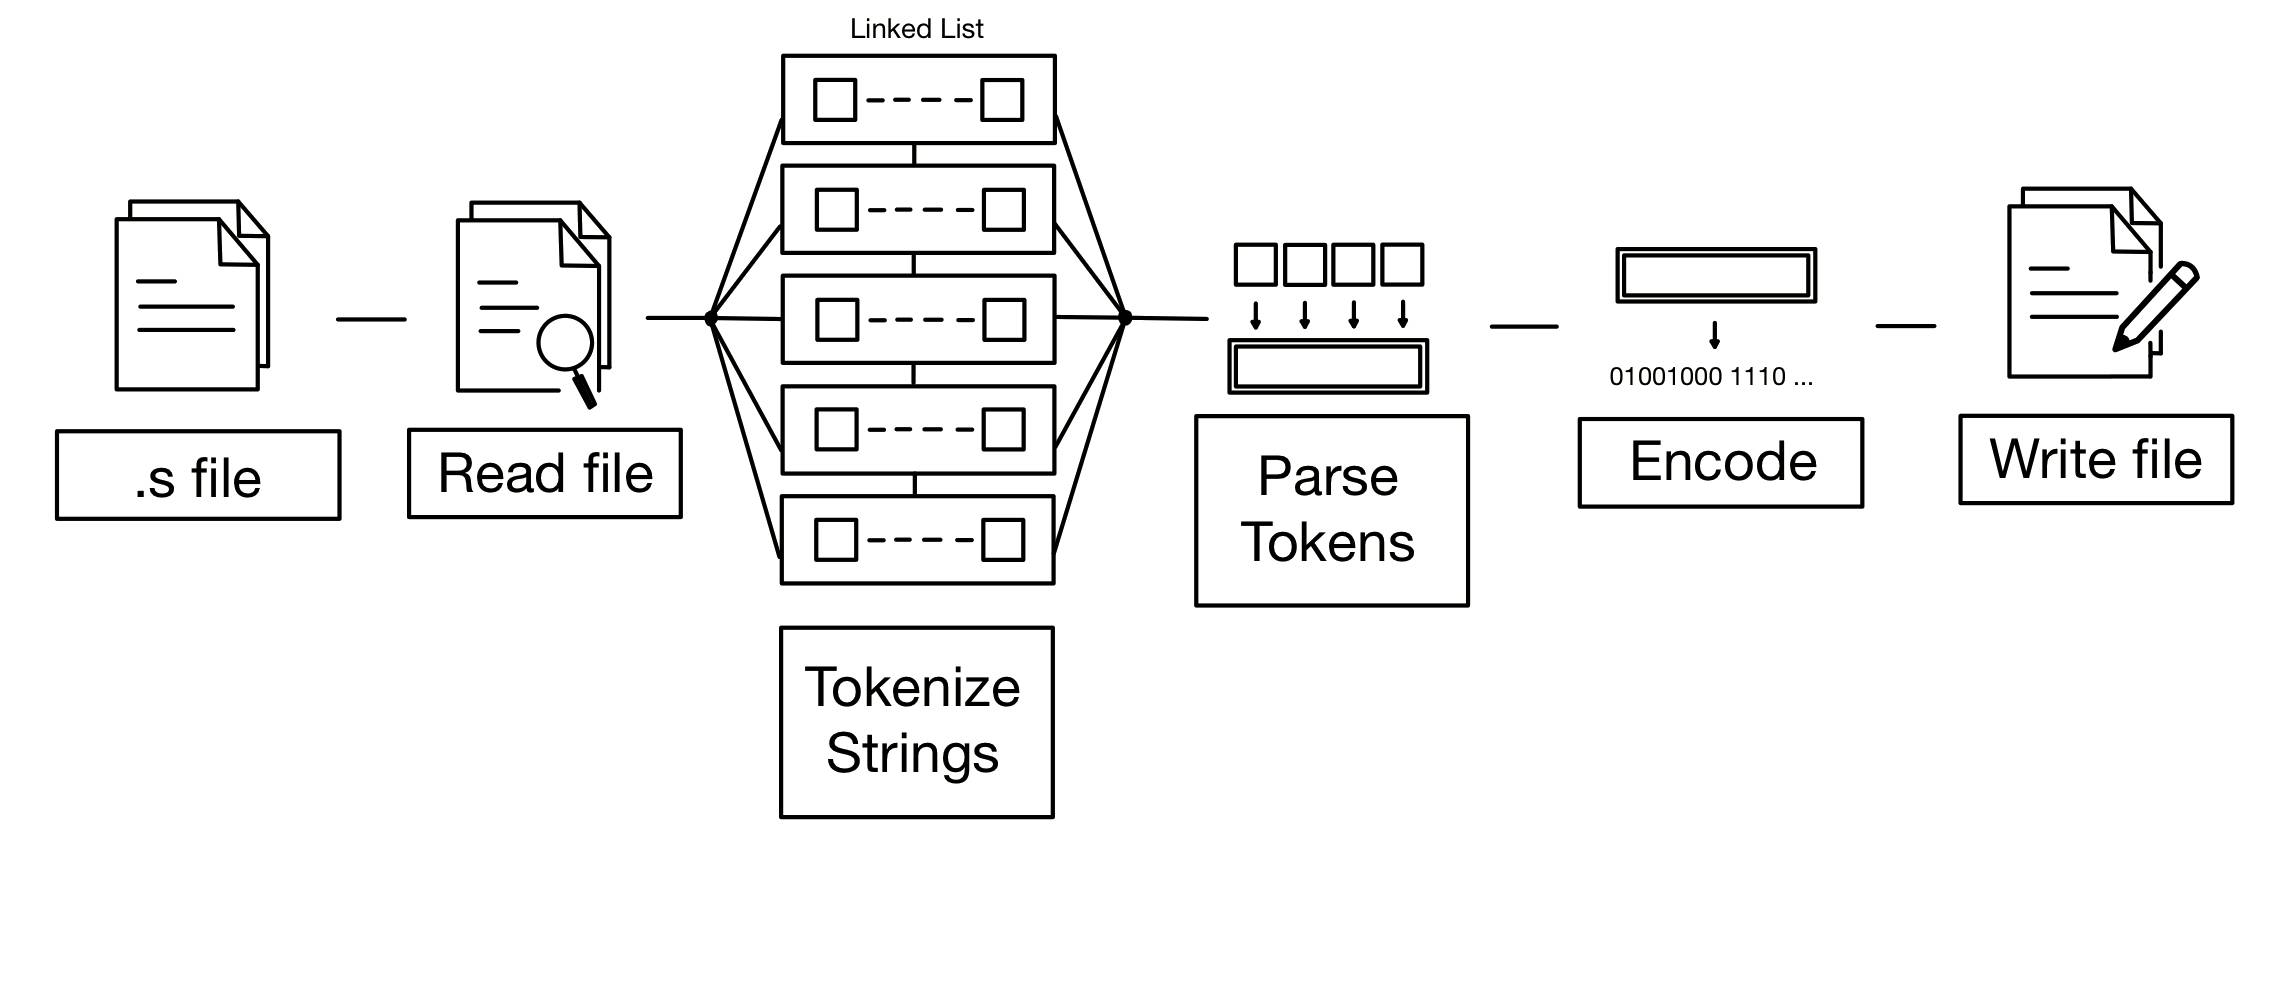
\includegraphics[width=15cm, frame]{assembler_flow.jpg}
    \caption{Our 2-pass assembly process}
    \label{fig:assembler}
\end{figure}

\subsection{The implementation:}\label{Assembler implementation}
\subsubsection{Problems we overcame: }
A notable issue we faced was that we did not know how many lines there were in each source file, so we could not create an array of strings to store these instructions. To tackle this, we used a linked list to store the instructions instead. Since we took such an approach, we could then read through the source file once, converting each instruction in a tokenized form and inserting them into the linked list. Labels are inserted into our symbol table, and are not inserted into the linked list. This is the reason why we preferred a 2-pass approach over a 1-pass one.

\subsubsection{Improvements after weekly meetings: }
During our weekly mentor meetings, Professor Knottenbelt suggested that we move away from switch-case statements and delve into the world of functional pointers. We took the advice and incorporated suitable function pointers wherever possible. Figure \ref{fig:functional_pointers} shows how we have used functional pointers in our assembler, this example shows that the function attribute of the instruction function map points to the appropriate function which is \verb|parse_dataproc| in this case. The use of this method allowed for code modularity and also enabling object oriented programming features in our code base.

\begin{figure}[htp]
\centering
\begin{BVerbatim}
instr_func_map and = {
.code.dataproc_opcode = AND,
.function = &parse_dataproc /* FUNCTIONAL POINTER USED */
};
// continues for all operations below...
\end{BVerbatim}
\caption{Example of functional pointers in the assembler}
\label{fig:functional_pointers}
\end{figure}

\subsubsection{Tokenizer:}
Another interesting aspect of our assembler is how our tokenizer works. Before passing anything to \verb|tokenizer()|, we check that its not a label, it will always be an instruction line. Then we allocate contiguous memory to a \verb|token_list| which will store our tokenized instruction. Then, instead of using \verb|strtok_r()|, we used our own version - \verb|strbrk_r|. This choice was made due to 2 reasons:
\begin{enumerate}
    \item \verb|strtok_r()| isn't portable for pre-POSIX-2001 systems and it caused a lot of compilation issues on macOS.
    \item Our \verb|strbrk_r| functions returns the delimiters inside the returned tokens, which was important to identify pre-indexed and post-indexed instructions. For example, \verb|strtok_r| wouldn't return the \verb|[]| in \verb|ldr r1, [r0]| and our program required that identification later on in the assembler process.
\end{enumerate}
Once we ran a \verb|while| loop inside \verb|tokenizer()|, we freed any memory allocation we may have used and then passed the tokenized list of type \verb|token_list|. This token list is then parsed and encoded as mentioned before.

\section{Extension: Modelling a Distributed Ledger Cryptocurrency with a Concurrent Centralised Network}
\subsection{Real world usage:}
\lipsum[1-1]
\subsection{The implementation:}
\lipsum[1-1]
\subsection{Testing:}
\lipsum[1-1]
\subsubsection{Effectiveness of testing:}
\lipsum[1-1]

\section{Group Reflection}
\subsection{Effectiveness of communication and division of work:}

% Division of work: Linked list (Kavya), Symbol table (Yelun), Tokenizer (Ash & Sid)
% Daily meetings to catch up on progress.
% Suitable branching to effectively divide work.
% Mostly detailed merge requests
% Doxygen comments to properly document code for future purposes

As discussed in the Emulator Interim Checkpoint, we have been using our Discord server for all our communications (text, audio and video). Our setup was more than successful in our opinions, it was the perfect balance of professional and casual as we were mindful of dividing our time between work and leisure. Whether it be late night talks about the countries we come from or sending memes in our \verb|#random| channel. During our almost 24/7 text correspondence, we spend approximately 6 to 8 hours on call to program, relax, make design decisions or brainstorm extension ideas. We are also very careful that we don't strain ourselves so we make sure that we collectively take breaks, which has in fact increased our productivity generally. In the assembler implementation phase of our project, we considered using a more thought out process of collaboration; we came across the concept of pair programming. This technique has a \textit{driver} (one who writes the code) and an \textit{observer} (one who reviews each line of code typed by the driver). It really helped us understand the code better, which in turn meant we could optimise/ refactor it easily. It also reduced the number of errors per line.

In the assembler, we decided to split up larger parts of the project. Kavya was in charge of creating the linked list which is essentially the backbone of the assembler, Yelun was in charge of the symbol table and Ashvin and Siddhant were in charge of the tokenizer. This way, we could essentially branch out from \verb|master| and then merge all branches together and fill any cracks we neglected. This method saved us a lot of time as everyone was independently coding at their own pace (which also allowed everyone to make suitable unit test cases in \verb|testrunner.c|). Another effective technique we used was making meaningful commit messages and merge request descriptions which come handy when we want to clarify a merge conflict or any gaps in understanding. Overall, we are all very happy with how well we have done in the project and the amount of progress we have made both as a team and personally.

\subsection{Future improvements:}
%
%
%
%
%
%

\section{Individual Reflections}
\subsection{Ashvin:}
\lipsum[1-1]
\subsection{Kavya:}
\lipsum[1-1]
\subsection{Siddhant:}
Overall, I am very satisfied with our project as it is the product of self motivated and guided work. Recalling back to the first 2 days of the project, some of us didn't know how to handle git branches and merge requests; so to see how far we have come since then is very rewarding. Not only did we finish the ARM emulator and assembler in time but we also incorporated the optional test cases. Our chemistry as a group worked very well because we set aside enough time in the day to bond as friends and not just teammates. This allowed free flowing conversations during brainstorming meetings and also enabled everyone to speak their mind freely without feeling anxious especially in a time like this where none of us have ever met each other in person.

As some members of our team had previous experience in industrial programming, they imparted that knowledge with the rest of us which encouraged good coding and git practices (like properly formatted git commit messages which convey suitable amounts of information within 1 sentence). I will definitely be carrying forward these valuable soft skills in future projects and hopefully in the workplace. If I were to do this project again, I would probably further divide the work for Assembler as pair programming held us back in terms of time, on the other hand, pair programming reduced the number of bugs we had during testing as there were 2 pairs of eyeballs on 1 piece of code.

\subsection{Ye Lun:}
I have participated in group projects for development in the past. These were all with supervisors, observing my work consistently and guiding me, to the point of hand holding. This C group project was one without such a supervisor. Most of the guidance from our mentor centered around improving what we already had accomplished. The initial project structure, and many other aspects were decided by ourselves. Making these decisions was a difficult yet fulfilling experience as we did not know what was optimal or not. Eventually, I understood that it is better to attempt to do rather than contemplate about hypothetical situations, since ultimately anything can happen.

Throughout the project, I learned to work better in group form. Our work in the emulator is rather segmented, we discussed the work we will do, and each member will proceed to work on their own isolated segment. In the end we put everything together to produce a result. When we worked on the assembler, we initiated more pair and group programming sessions so we could understand what one another is doing in real time, rather than when we were reviewing code. Our group cohesiveness improved and this carried over into building our extension. I will certainly bring this practice into future group projects and recommend it to others.

\end{document}